\documentclass{below-ext}

\title{A standard for Home monitoring}

\numberofauthors{4}
\author{
  \vspace{-1.5em} 
  \alignauthor{
  	\textbf{Patrick Hendriks}\\
  	\email{patrick.hendriks@hva.nl}
  }
  \vfil
  \alignauthor{
  	\textbf{Mats Otten}\\
  	\email{mats.otten@hva.nl}
  }
  \vfil
  \alignauthor{
  	\textbf{Suzanne Peerdeman}\\
  	\email{suzanne.peerdeman@hva.nl}
  }
  \vfil
  \alignauthor{
  	\textbf{Glimworm IT BV}\\
  	\affaddr{Kattenburgerstraat 5}\\
  	\affaddr{1018 JA Amsterdam}\\
  }
}


% Paper metadata (use plain text, for PDF inclusion and later re-using, if desired)
\def\plaintitle{A standard for Home monitoring}
\def\plainauthor{Patrick Hendriks; Mats Otten; Suzanne Peerdeman}
\def\plainkeywords{Ambient environment; Elderly care; Healthcare technology}
\def\plaingeneralterms{Research}

\hypersetup{
  % Your metadata go here
  pdftitle={\plaintitle},
  pdfauthor={\plainauthor},  
  pdfkeywords={\plainkeywords},
  pdfsubject={\plaingeneralterms},
  % Quick access to color overriding:
  %citecolor=black,
  %linkcolor=black,
  %menucolor=black,
  %urlcolor=black,
}

\usepackage{graphicx}   % for EPS use the graphics package instead
\usepackage{balance}    % useful for balancing the last columns
\usepackage{bibspacing} % save vertical space in references
\usepackage{ragged2e} % alignment
\usepackage[utf8]{inputenc}
\usepackage[english]{babel}
\usepackage{lipsum}
\usepackage{epstopdf}
\usepackage{amssymb}
\usepackage{pifont}% http://ctan.org/pkg/pifont
\newcommand{\cmark}{\ding{51}}%
\newcommand{\xmark}{\ding{55}}%

\begin{document}

\maketitle

\begin{abstract}
In this paper the team of BeLow set out to explicate the gap between the demand for monitoring technology for the elderly, and the actual grasp upon the market. Initially a continuation of the Healthy Life Lamp project by Sven Erik Haitjema, BeLow leaned more in the direction of a portable living lab rather than one central monitoring device. 
\end{abstract}

\keywords{\plainkeywords}
\category{H.5.m}{Information interfaces and presentation (e.g., HCI)}{Miscellaneous}. 
%\terms{\plaingeneralterms}

% =============================================================================
\section{Introduction}
% =============================================================================
For the past several years, the changing demographic in the Netherlands has raised many concerns. The growing number of elderly people living alone and the question of how to care for the ageing population have caused a surge of technological developments aimed specifically at this target audience. However, even if a demand for ambient intelligence based systems such as these, the market does not quite seem to take off in the way that most developers hope for. Conduction of several focus groups among elderly people living independently has proven that the demand exists, yet is often not satisfied by what is currently on offer. Various systems target the caregivers of those that will actually be using the product, rather than the users themselves. It has become apparent that a large portion of the elderly population wishes to be respected in their autonomy, and take matters into their own hands.\cite{cbs_households}

\begin{figure}
\center
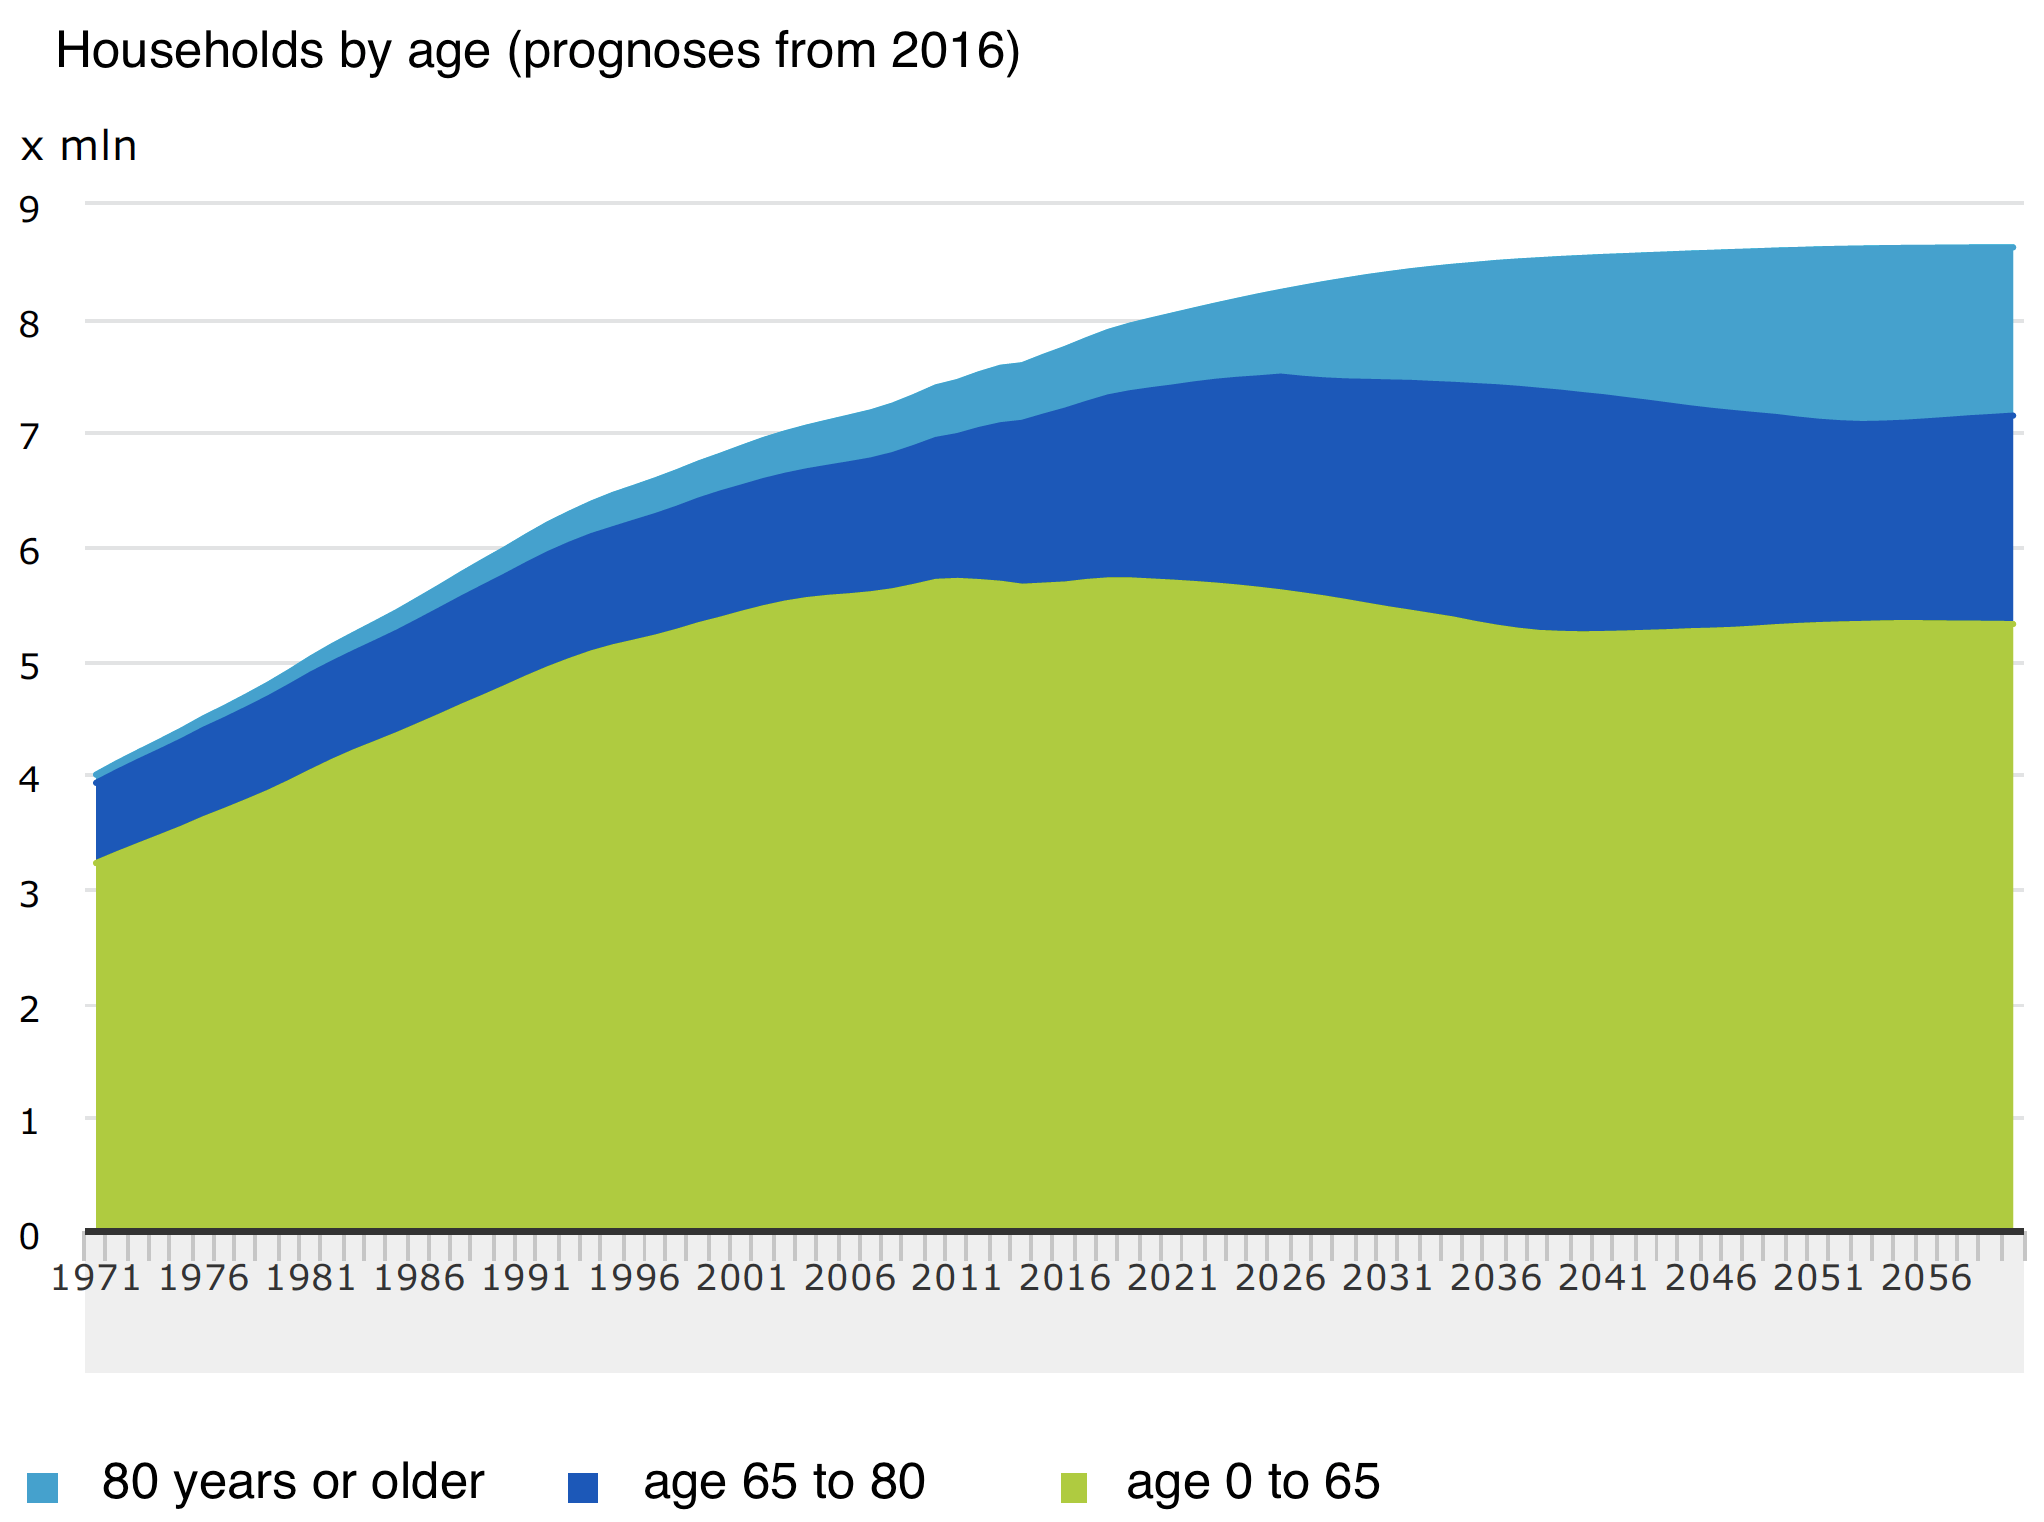
\includegraphics[width=0.5\textwidth]{cbs_household_age_report}
\caption[Translated graph]{Translated graph from CBS\footnotemark }
\end{figure}
\footnotetext{Central bureau of statistics of the Netherlands}
The products available are also specifically targeted at an elderly audience, even though they would be able to cater a much more diverse group of users. Therefore, the goal of BeLow is to lay the foundation for a portable living lab; a standard kit that can be used by anyone, even those with minimal technical experience, and that can be expanded upon by those that wish to do so.

A major part of this research was performed within Stedeborgh; a living community by the elderly for the elderly. Stedeborgh is a largely autonomous community, with residents aged 67 and up. For this paper several tests, focus groups and interviews were conducted among the residents, and their sentiments, routines and opinions have played a big part in the decisions that were made. Aside from Stedeborgh, this research was performed in collaboration with Amsterdam's Digital Life Centre's project BRAVO (led by Saskia Robben, 1 Apr 2016 - 1 Apr 2018) and Glimworm Information Technology (Adrian Blackwood). Collectively, the question we ask ourselves is: "How can we develop an accessible standard with which to add a layer of intelligence to the living environment?" 

In this paper the focus will be on answering the aforementioned question, as well as answering several other questions:
\begin{itemize}
\item What monitoring systems are currently on the market, and what knowledge is available?
\item  What are the wishes of the target audience when it comes to improvement of living quality using technology?
\item How can the needs of the target audience be satisfied using technology.
% Weet niet of we deze in de huidige vorm zo zouden moeten laten staan. De 3 punten erboven vind ik beter aansluiten. \item How does one become a standard?
\end{itemize}
%hieronder wordt nu geplaat over first two and second half. zin moet vanwege hierboven dan ook aangepast.
This paper will begin with a report on literature and field studies performed to answer the first two of these questions. The second half will consist of reports on experiments and tests performed using prototypes. Finally, we will look to the future and, based on interviews with experts on the subject, discuss how technology may develop in the years to come and how this can be of use to society as a whole.


% =============================================================================
\section{Related Work}
% =============================================================================
This section will focus on the state of the art technology as of this time (2017), as well as the current situation of Elderly care for senior citizens that are living independently or semi-independently in living groups. The first half of this section will illustrate how the care and national budget for this care are managed, what tools are frequently being used and what gaps are currently being encountered. Furthermore we will investigate how independent living groups have developed their own systems for keeping everyone healthy and autonomous. The second half of this section will briefly summarize the current state of the art technology, what advantages they offer the user, and what disadvantages are being encountered.



% =============================================================================
\subsection{Care for independent senior citizens}
% =============================================================================

A surprisingly big misconception when it comes to innovation aimed specifically at the elderly community, is that this is an audience that, as a whole, wants roughly the same thing; all share similar fears, weaknesses and requirements. In reality, however, there exists a myriad of different people all with different abilities and disabilities. Some are physical, such as bone atrophy, or mental, such as dementia or a combination of the two resulting from a stroke. [Reitenbach and Schot, 2012]  As of 2015, the government of the Netherlands has aimed to reform the long-term care for the elderly in such a way that more responsibility is given to the able citizen. This changes the nature of the long-term care program to that of a package of care and support which the active population, using their own resources, can call upon in order to maintain their autonomy and age with dignity.[Campen, Iedema, Broese van Groenau and Deeg, 2017]

The policy in the Netherlands and other European countries strives to enable elderly citizens to grow old in their own home and/or neighbourhood (aging in place) by use of their own resources and a package for care and welfare facilities. \cite{thomas_blanchard} Despite the best efforts of fellow citizens and caregivers however, this method does not always suffice and, more importantly, does not give the loved ones of the elderly citizens in question peace of mind. This is where electronic monitoring systems get to play their part.


% =============================================================================
\subsection{Electronic monitoring for the elderly}
% =============================================================================
Electronic monitoring of elderly and/or vulnerable citizens is nothing new, there is a myriad of systems available that offer various degrees of support to the user. These vary from wearables that either monitor or aid the user, or both. Take for example the Lechal insoles: "Owned by the India-based company Ducere, Lechal offers a line of smart shoe inserts to help visually impaired wearers more easily navigate the world at large. These smart insoles provide directional assistance in the form of gentle vibrations and phone notifications, giving seniors a greater degree of independence. The associated app also allows for location sharing, letting you keep tabs on your loved one no matter where they are." \footnote{quoted from safewise.com} A simpler solution would be monitoring wearables similar to fitbits, which keep tabs on the user's heart rate and blood pressure, or simply a wearable alarm button which notify emergency services when pressed.

Of course, these are all relatively simple systems focusing on one particular element, but there are also various platforms available on market. In the spring of 2016 Philips introduced CareSensus, a sensor platform created in collaboration with Right At Home, one of America's biggest franchises for  home care services. This system was later deployed in the Netherlands by Cordaan, a major home care institution in Amsterdam, to aid people suffering from dementia. CareSensus proved the potential succes of deploying various sensors in the living environment for health monitoring.

There are several similar platforms available such as:

\begin{itemize}
\item Care@Home van Essence
\item Sensara
\item Livind
\end{itemize}


% =============================================================================
\section{Pre-design research}
% =============================================================================

\subsection{Stedeborgh}

Before the creation of the prototype we visited Stedeborgh, an independent living community for the elderly, to gather some first hand insights and information. Stedeborgh is an independent living community situated in Grootebroek, the Netherlands.  It is not your standard nursing home; it is for the elderly, by the elderly. The residents live alone or in couples in fully fledged apartments, meaning each apartment has its own kitchen and bathroom as well. The apartments face to the inside of the complex, rather than to the outside, and are connected by an indoor garden featuring tropical foliage and equally tropical temperatures. on the ground floor is a large entertainment hall which is perfect for get-togethers, and a cafeteria for special events. The complex is surrounded by a lovely community garden. What makes Stedeborgh stand out most, however, is the way in which the residents look out for each other.

\subsection{Systems}
The community is maintained by its residents, which means that everyone has a task and responsibilities within the community. A number of systems has been put in place to ensure the safety an wellbeing of the residents. The system that inspired us most was the "asleep/ awake" system. Every apartment has a sign on the door with a sun on one side, and a moon on the other. This sign is turned accordingly whenever the residents go to sleep, and whenever they wake up in the morning. The residents take weekly shifts in which they pass by all the doors in the evening and first thing in the morning. If a sign has not been turned appropriately this could be an indication that something has gone wrong, and the appointed member of the community will check up on their peer immediately. This method, however simple it may be, has proven to be very effective in solving one of the major concerns when it comes to the safety of elderly people living alone; injury by fall. Countless accounts exist of elderly people falling down within their own home, and being unable to get up. In the worst of these cases, the victim may spend days incapacitated on the ground without anyone coming to their aid, sometimes even with death as a result. The system in Stedeborgh ensures that the residents, at the very least, are not without aid for longer than eight hours. 

\subsection{Stedeborgh as a target audience}
As we were inspired by this community's way of life, and the living quality of its residents, we decided to make the residents of Stedeborgh our main target audience, and design our use cases for this research around them. We were curious about their stance on the use of technology for health-monitoring, and what would make such a system attractive to them as individuals, and as a community. We made the decision to conduct a focus group among those that were interested in our research.

% =============================================================================
\section{Focus group}
% =============================================================================

As part of our research, we conducted a focus group at Stedeborgh among a group of volunteers. The group met in the cafeteria where they were provided with coffee, tea and sweets. We strove to keep the atmosphere as casual and relaxed as possible, to encourage the participants to speak freely and openly about the subject. The participants were introduced to BeLow and, surprisingly enough, did not require too much explanation. Whereas most of the performed desk research concluded that the elderly population of the Netherlands was near phobic of technology, the residents of Stedeborgh proved the contrary: many were already familiar with several systems on market today, and some even owned their own.

\subsection{Stigma}
 One of the older participants, a lady nearing her 90's, told the group she always had her alarm button with her, attached to her walker. The woman had trouble walking due to bone atrophy, but was still living independently. When asked about the stigma devices such as these carry, she responded casually: "I am an elderly woman, at my age no one should feel ashamed about carrying a device that helps them in case of emergency. You all have your cell phones too, don't you?" She also told us that the device has thus far helped her maintain her autonomy to quite an extend. She has not yet had a falling incident, but she is very well aware of the fact that she is at risk. The alarm button gives her a sense of security that has given her the confidence to continue doing the things she does. Because if she were to fall, she would be able to immediately call for aid. The majority, if not all of the respondents, agreed with her.

\subsection{Monitoring}
During this first discussion the respondents expressed a clear wish for products such as the one BeLow aimed to develop. We were told that commercial parties had come by several times already to offer their services and products. When asked for the main reason why there was never an investment in these products, the respondents had two very clear reasons. Firstly, the price point; many of these products came with a hefty pricetag. Stedeborgh is an independent community run mainly by its residents, and it simply couldn't afford to spend up to thousands of euros on products that piqued their interest, but had not yet proven their worth to the community's satisfaction. More importantly, however, the respondents stressed the fact that the systems often lacked transparency. Many of the presented solutions made use of cameras, which aroused a sense of uneasiness in the users. One man told us that even though he was ensured that the visual data captured would be analyzed by algorithms rather than people, this did not take away the feeling of being watched. "The word algorithm doesn't give me any idea of what is happening inside," he said half jokingly. "If you tell me an algorithm is analyzing my video feed, you might as well just tell me a midget or a ghost is watching me." Many of the respondents agreed that the systems were not transparent enough, and not only because they were described using terminology which did not resonate with them. Some even went as far as to admit the way the systems were designed made them feel like children being watched. "Most of these systems are made in such a way that they will provide reports about your well being to a caretaker or a doctor. I do not want that. If I am feeling under the weather I would much rather have my daughter calling me to see if I am doing ok than have a nurse rush in to usher me out of bed because I am 'not getting enough exercise'," one of the relatively younger women stated. 

\begin{figure}
\center
\label{fig:interview}
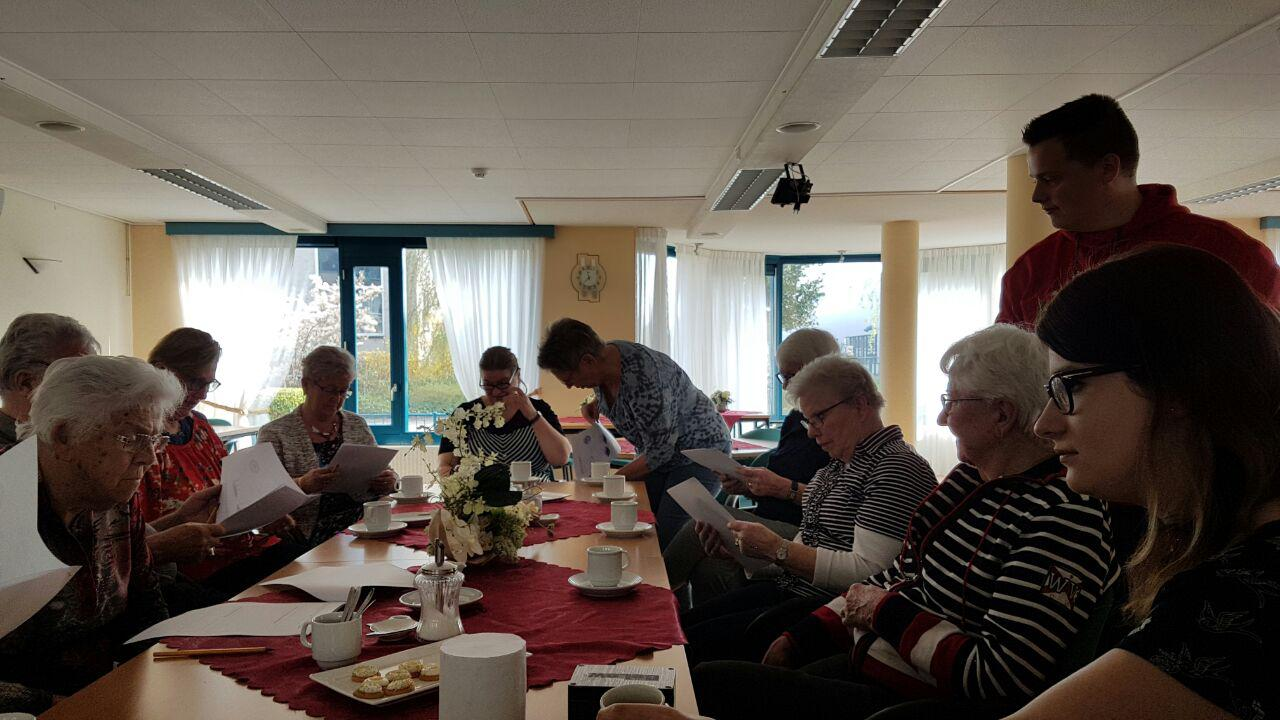
\includegraphics[width=0.5\textwidth]{interview}
\caption{Interview Group}
\end{figure}

\section{Technology}
Technologie heeft een hele hoop veranderd voor mensen hun dagelijks leven. Apparaten worden steeds kleiner en sneller, en ook worden deze steeds energie zuiniger ontwikkeld. Dit brengt een hoop nieuwe mogelijkheden met zich mee. Waar we 10 jaar geleden nog met telefoons die konden bellen en sms'en lopen de meeste Nederlanders nu met een smartphone op zak. Deze mobiele computer bevat ook steeds vaker een reeks aan sensoren waar voorheen vrij specialistische apparaten voor vereist waren. Ok toegegeven de kwaliteit en nauwkeurigheid met professioneel toegespitste elektronica laat nog wat te wensen, maar over het algemeen zijn deze sensoren heel goed bruikbaar omdat er niet altijd met zulke stricte foutmarges gewerkt hoeft te worden. Dit opent ook de deur naar goedkopere en toegankelijkere zorgtechnologie. 


%We kennen allemaal de toilet val alarmen waarbij er aan een touwtje getrokken moet worden wanneer iemand ten val komt. 
% nee die kennen we niet, leg uit
Tegenwoordig hebben ouderen ook de mogelijkheid een nekhanger te dragen die een alarmknop heeft. 
% wie heeft dit op de markt gebracht? hoe werkt dit? vermeld de bron
Dus nu hebben we de beperking van een bepaalde ruimte overwonnen door verbeterde technologieen. Met het sinds 2016 landelijk dekende LoRa netwerk is het nu ook mogelijk een alarmknop overal mee te nemen zonder bang te zijn dat de batterij misschien niet is opgeladen. In het het geval van ouderen is het nog geen gemeengoed dat zij ook een internetverbinding hebben laat staan eentje op zak. Hier komt mogelijk in de toekomst verandering in doordat de generaties van nu opgroeien met internet.
% Introductie technologie.
 
In onze studiegroep had niemand een internet verbinding. Mede om deze reden is er gekozen om gebruik te maken van de IoT\footnote{Internet of Things} LoRa\footnote{Low power Radio} techniek. Wat LoRa bijzonder maakt is dat het over lange afstand berichten over kan brengen zonder dat hiervoor een continue stroombron vereist is. Wel heeft LoRa een maximum te verzenden berichten per dag dan wel een beperkte bericht grootte. Bij dit onderzoek is er gebruik gemaakt van techniek die veelal passief de omgeving / proefpersoon in de gaten houdt. We maken hierbij geen gebruik van bijvoorbeeld camera's. Dit is zowel een belangrijk punt wat betreft de privacy en acceptatie voor monitoring systemen, maar ook doordat de sensoren die geplaatst worden normaliter op batterij werken. In het prototype is rekening gehouden met laag stroomverbruik. Zo hebben wij voor communicatie onderling tussen node en gateway gekozen voor een zeer veel gebruikte en bekende standaard namelijk die van bluetooth low energy. Doordat Bluetooth low energy in zoveel apparaten aanwezig zijn kunnen deze makkelijk aan een netwerk van sensoren worden toegevoegd. De data die opgehaald wordt van de sensoren wordt naar de gateway verstuurd. Deze gateway kun je het beste zien en omschrijven als een gewone internet router. Deze zorgt er namelijk voor dat de data buitenshuis komt, en uiteindelijk bij de Cloud terecht. Waarnaar de Cloud op beslissingen gebaseerd op algoritmes en voorkeuren een event genereerd en bijvoorbeeld de gebruiker zelf dan wel de contactpersoon bericht.

\begin{figure}
\label{fig:process}
\centering
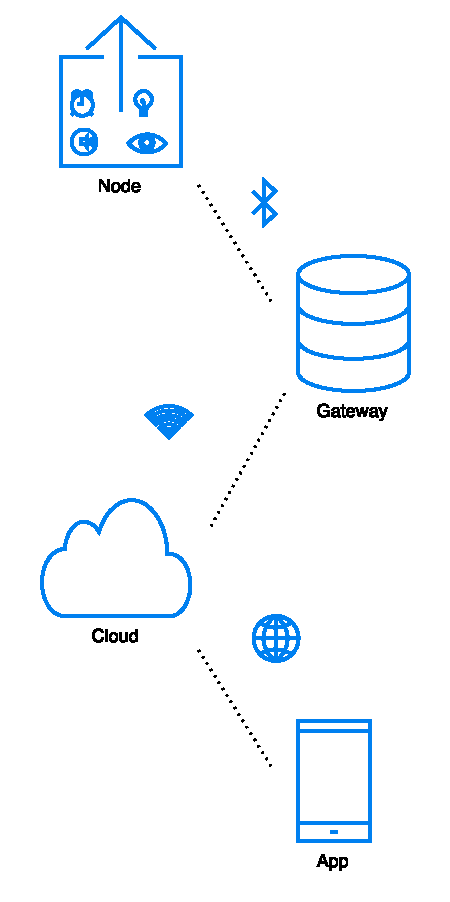
\includegraphics[scale=0.6]{dataproces.pdf}
\caption{Schematic of the data collection process}
\end{figure}

\subsection{Open standards}
% dit kan veel uitgebreider: wat is de toegevoegde waarde voor de ouderen, wat kan het mogelijk betekenen voor digital life centre, of geliefden van de doelgroep. Kan het studenten helpen (PORTABLE LIVING LAB) 
Met het gebruik van voornamelijk open standaarden willen we zorgen dat in de toekomst ontwikkelaars en hobbyisten zich willen bezig houden met het ondersteunen onderhouden en uitbreiden van de mogelijkheden. Zoals het platform nu is ingericht is er nog weinig spannends vast te leggen. Een van de toepassingen die we graag zien is om mensen te kunnen laten inter-acteren met het platform. Er voor kunnen zorgen dat het niet alleen voor zorg specialisten een handige tool is. Maar dat de mensen waarom het gaat er ook iets nuttigs in zien. Hoewel de Google Home en de Amazon Alexa geen (echte) open standaard zijn zou je wel kunnen denken aan een soort personal assistent die er ook voor zorgt dat je je pillen op tijd inneemt. Tegelijkertijd is er een sensor in de pillendoos die opmerkt dat ze inderdaad ingenomen zijn. Deze data is uitermate geschikt voor het platform en makkelijk toe te voegen.
\subsubsection{Data Proces}
\begin{figure}
\center
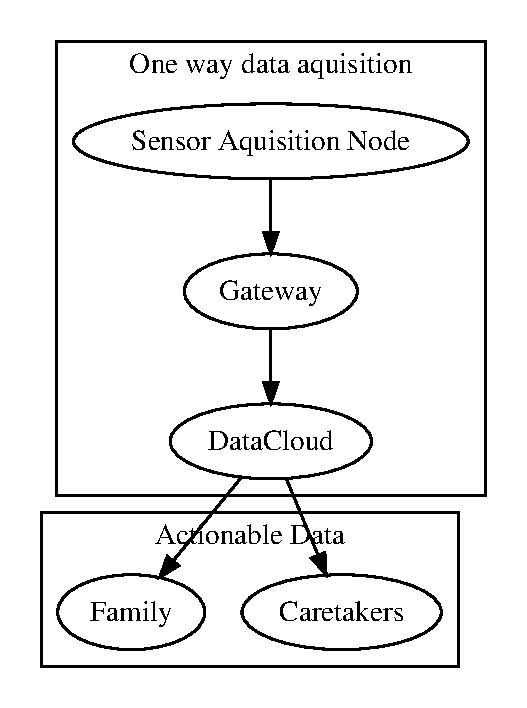
\includegraphics[width=0.2\textwidth]{process}
\end{figure}

%-----------------
\subsection{Goal}
Wat we met dit onderzoek willen bereiken is kijken of het mogelijk is de oplossingen die er zijn in de vorm van dure commerciële technologieën in de vorm van community based platformen te gieten. Tegelijkertijd moeten we ons ervan bewust zijn dat bepaalde specialistische hulp of technologie altijd nodig zal zijn. Met de in de laatste paar jaren steeds meer beschikbaar geworden platformen zoals Arduino, Raspberry Pi en de vele sensoren willen we gebruik maken van deze opties voor onder andere de zorg. De data die doorgaans met dit soort platformen vergaart worden zijn in bepaalde gevallen niet secuur genoeg om echt kennis uit te halen in individuele gevallen. Technologieën zoals Machine based learning bieden hiervoor een uitkomst. Zo kunnen er verbanden worden gevonden en aangetoond die er uiteindelijk voor zorgen dat data bruikbare informatie wordt. Ons platform bied een methode om heel veel data te vergaren. Met specialisten, machine based learning en onderzoekers is het uiteindelijk de bedoeling om dit om te vormen naar informatie, kennis en wijsheid\ref{fig:dikw}. Wanneer we deze kennis bezitten kunnen we veel beter preventief te werk gaan dan puur alleen registeren van gebeurtenissen. Het gebruik van dit platform moet er dan niet alleen voor zorgen dat de kosten van de zorg afnemen maar dat er ook beter gelet wordt op de wensen van hulpbehoevenden. Het aantal fouten wat gemaakt wordt door menselijk handelen is hierdoor te verminderen. Ook is een computer zich beter bewust van subtiele veranderingen dan dat mensen dat kunnen waarnemen. 
\begin{figure}
\center
\label{fig:dikw}
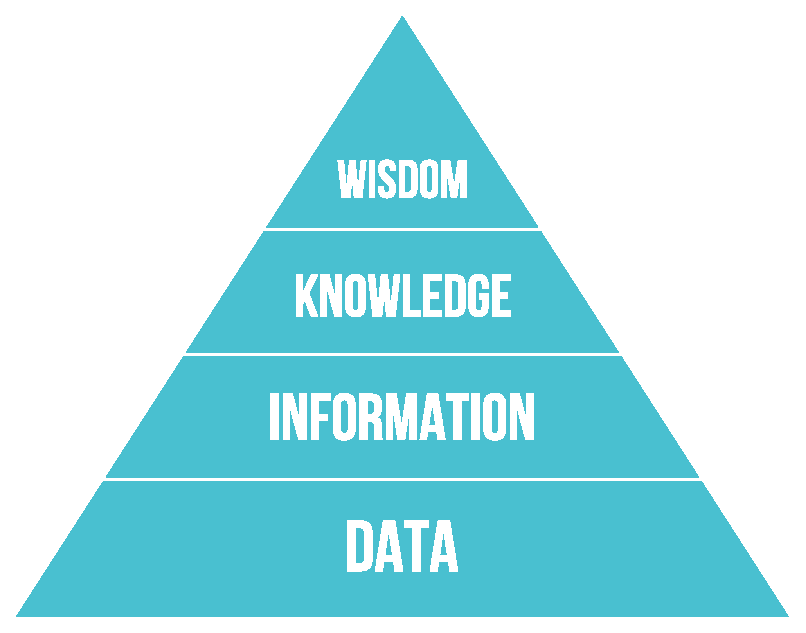
\includegraphics[width=0.4\textwidth]{dikw}
\caption{Data Information Knowledge Wisdom model}
\end{figure}
\section{What we have done}
In dit onderzoek zijn we uitgegaan van een technologische oplossing die voornamelijk familie en verzorgers op de hoogte houdt wanneer er iets (mogelijk) fout gaat. Wat we wilden bereiken is dat mensen zelf de touwtjes in handen krijgen
\subsection{Room monitoring}
\begin{figure}
\label{fig:floorplan}
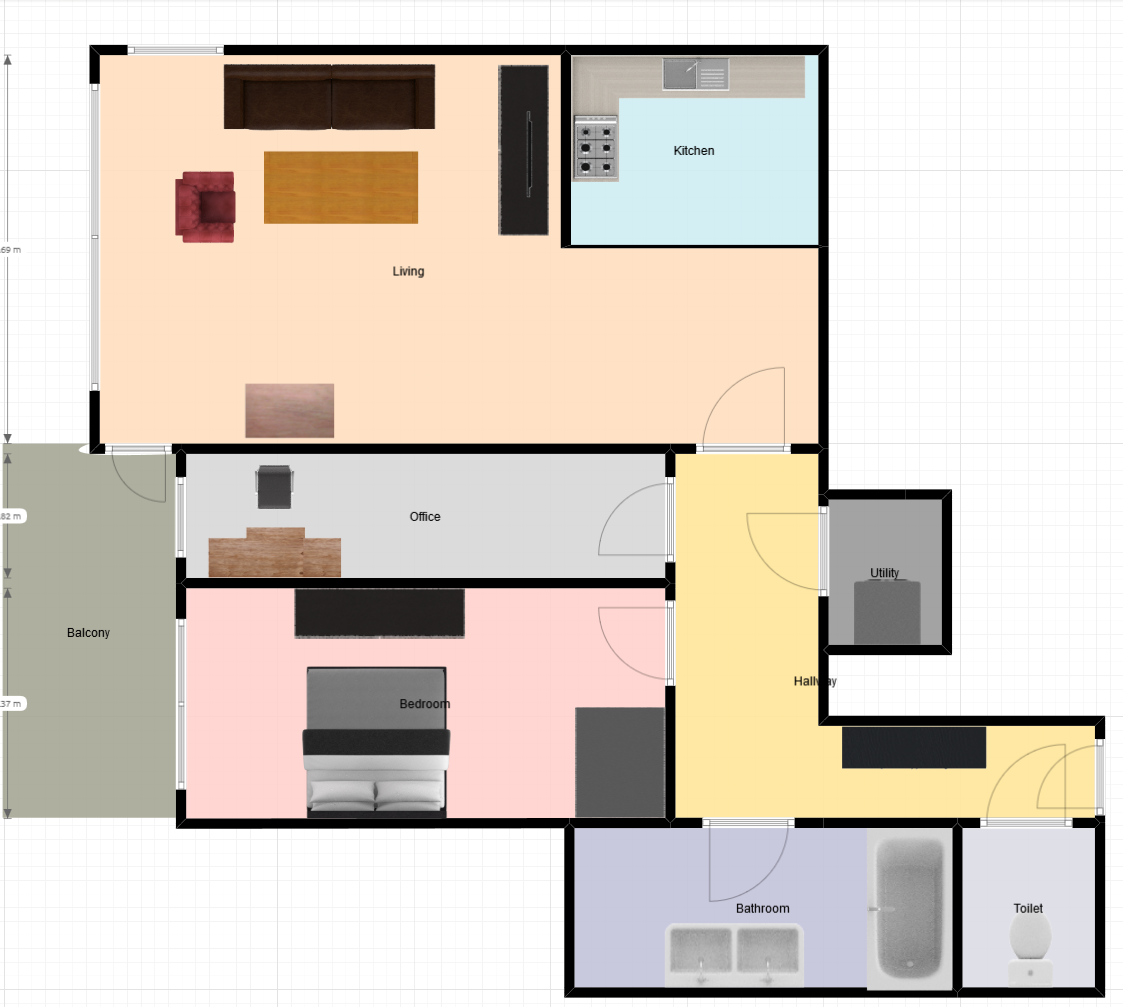
\includegraphics[width=0.4\textwidth]{floorplan.png}
\caption{Floorplan of field-test}
\end{figure}
Bij figuur\ref{fig:floorplan} hebben we 3 gebruikt die data verzamelde. De sensoren waren op een strategische plek geplaatst om de meest interessante data te bemachtigen.
\section{Data analysis}
\section{Conclusion}

\section{Future work}
Wat er in dit onderzoek nog niet gebeurd is, maar wat wel duidelijk naar voren kwam bij de interviews is het terugkoppelen van data. Zo wordt er veel aandacht besteed aan het koppelen van data en gedragingen van de personen in kwestie. Maar de personen krijgen deze data zelf niet te zien. In plaats daarvan krijgen ze adviezen van medisch specialisten wanneer deze ook al sneller en beter gepresenteerd zou moeten kunnen worden bij de persoon zelf. Hiervoor is wel vereist dat er een makkelijk te begrijpen interface wordt bedacht die deze mensen in staat stelt met die informatie zelf hen gedrag kunnen aanpassen.
%\subsection{Security}
%In het onderzoek in alleen gekeken naar de functionele requirements die bij een monitoring systeem komen kijken. We hebben gedacht aan security maar gekozen om dit in het prototype niet te verwerken vanwege de beperkte duur van het onderzoek en beveiliging moet goed geïmplementeerd worden en is geen klus die zo even geklaard wordt. blablabla WIP\ldots
%\subsection{Two way communication}
%Doordat er via LoRa maar een beperkt aantal berichten per dag verstuurd mogen worden, en LoRa zich minder goed leent voor twee weg communicatie is een 3g of 4g modem wellicht een betere keuze.
\balance
\bibliographystyle{acm-sigchi}
\bibliography{refs}
\end{document}
